\documentclass{article}
\usepackage[T1]{fontenc}
\usepackage{lmodern}
\usepackage{graphicx}
\usepackage{amsmath,amssymb}
\usepackage[a4paper,margin=2cm]{geometry}
\usepackage[absolute,overlay]{textpos}
\setlength{\TPHorizModule}{1mm}
\setlength{\TPVertModule}{1mm}
\usepackage[indonesian]{babel}
\usepackage{hyperref}
\setlength{\emergencystretch}{2em}
% unit: Halaman 53

\begin{document}

% === Halaman 53 (llm) ===

\vspace{250.07mm}

\section*{Kriptografi pada Bangsa Arab}

Sejarah kriptologi pada bangsa Arab dapat dibaca pada seri buku \textit{Arabic Origins of Cryptology} yang diterbitkan oleh \textit{King Faisal Center for Research and Islamic Studies}, Arab Saudi.

\vspace{40mm}

Ibn ad-Durayhim bernama lengkap Ali ibn Muhammad ibn Abd al Aziz, Tag ad-Din. Dia lahir di Mosul, Irak, pada bulan Sya'ban tahun 712 H atau 1312 M. Dia sering berdagang antara Kairo dan Damaskus dan ditunjuk sebagai guru di Masjid Umayah Damaskus. Dia pindah ke Mesir tahun 760 H/1359 M dan dikirim oleh Sultan sebagai duta kepada raja Abyssinia (sekarang Etiopia).

% deskripsi: Sampul buku berjudul 'Arabic Origins of Cryptology Volume Three: ibn ad-Durayhim's Treatise on Cryptanalysis'
% bbox normalisasi: [0.6120, 0.0340, 0.9570, 0.8760]
\begin{textblock*}{72.45mm}(128.52mm,10.10mm)
\noindent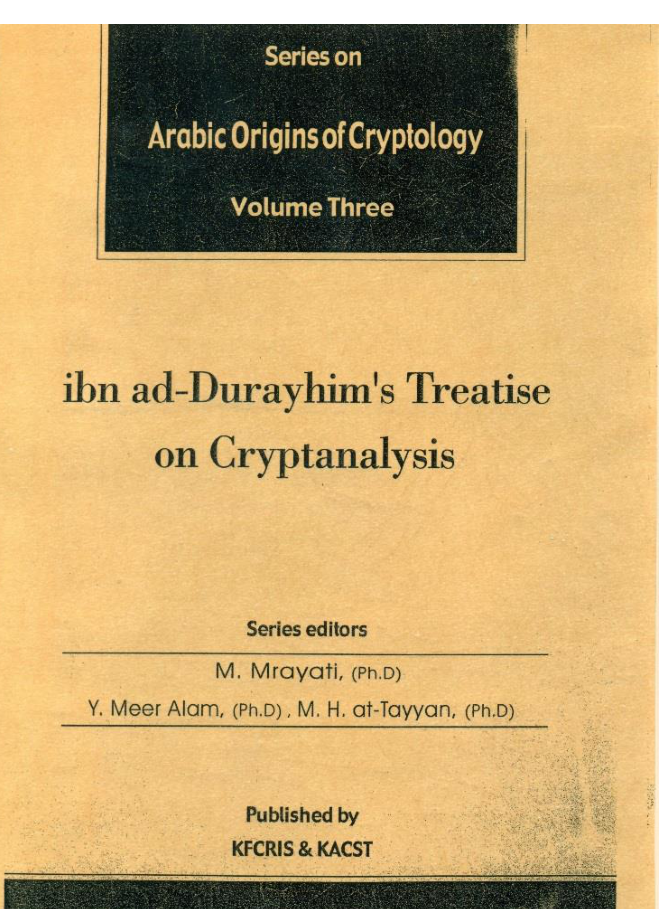
\includegraphics[width=72.45mm,height=250.07mm]{../../images/llm/page_053_img_01.png}%
\end{textblock*}

\end{document}
